\chapter{Literature Review}
% -------------------------
%% QUOTE
\vspace*{\fill}
\epigraph{Those who don't know history are destined to repeat it.}%
{\textsc{Edmund Burke}}
\clearpage{\thispagestyle{empty}\cleardoublepage}
%%
%% Body of the chapter
%%%%%%%%%%%%%%%%%%%%%%


\section{Overview and properties of gel systems}

A gel-system, as referred to in this work, is a polymer solution that has gone through gelation to form a highly viscous and immobile material in the porous formation. The properties of gels in terms of their basic chemistry are discussed in this section, and general overview about polymers is introduced.

Polymer, as a word consists of two parts: “poly” (many) and “mer” (parts) . A polymer is a macro-molecule that is made of repetitive smaller molecules, referred to as monomers, which are either covalently or ionically bonded. Despite the simple concept of polymers, it was not accepted until late 1930’s, as Hermann Staudinger laboratory results were successful in synthesizing polymers, and obtained because of it the Noble Prize in Chemistry in 1953 \citep{Roberts1977}.

Polymers have different physical and mechanical properties compared to their original
monomers. This is due to the significant difference in the length to diameter ratio between the polymer and its original monomer constituents \citep{Ghosh2006}. Figure \ref{fig:polymer} shows a polymer molecule composed of small monomers.

\begin{figure}
    \centering
    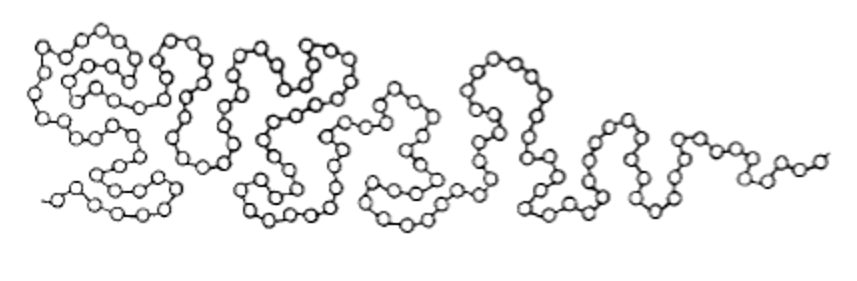
\includegraphics[width=\textwidth]{img/fig/polymer.png}
    \caption{Polymer consisting of several attached monomers (circles) \citep{Ghosh2006}}
    \label{fig:polymer} % 2.1
\end{figure}

Figure \ref{fig:polymonomer} shows a synthetic polymer, referred to as polyacrylamide (PAM) which is one of the most applied polymers in conformance enhancement operations due to its low cost and its good viscosifying properties \citep{Kabir2001}. The monomer (left) can be repeated multiple times in the sequence of the polymer (right) to obtain the desired properties.

\begin{figure}
    \centering
    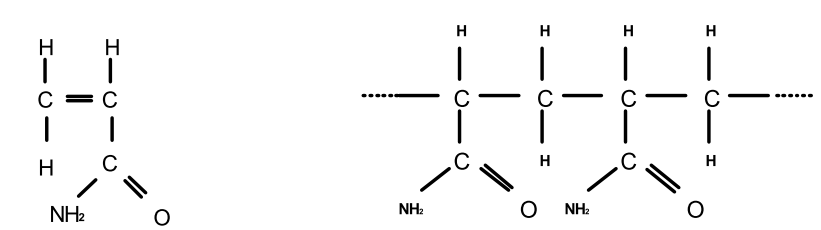
\includegraphics[width=\textwidth]{img/fig/polymonomer.png}
    \caption{Monomer: Amide (left) and polymer: polyacrylamide (right) \citep{Kabir2001}}
    \label{fig:polymonomer} % 2.2
\end{figure}

\subsection{Gel system types}

Gels can be divided into organic and inorganic. Inorganic gels include silicate-based, and Al(III)-based. Organic polymers can be classified in different ways, e.g. based on their origin, thermal response, mode of formation, line structure, physical properties, tacticity, and crystallinity \citep{Ghosh2006}. In the petroleum industry, organic polymers are often classified based on their origin. This includes natural polymers, i.e. biopolymers such as Xanthan and Scleroglucan \citep{Al-Muntasheri2012}, and synthetic polymers such as polyacrylamides, which are usually used in their partially hydrolyzed form, hereafter called HPAM \citep{Finch1992}. This report only addresses organic gel systems.

Polyacrylamide-based polymers have been used largely in water diversion operations throughout the history of the petroleum industry due to their low cost comparted with other gel-systems, and due to the good mechanical strength of the formed gel. 

\subsection{Polyacrylamide based gels}
Throughout the history of the petroleum industry, polyacrylamide-based gels were most commonly used in water diversion operations \citep{Al-Muntasheri2005, Ball1984} (Al-Muntasheri et al. 2005; Ball and Pitts 1984). In chemistry, acrylamide can be referred to as acrylic amide. Figure \ref{fig:acrylamide} shows the chemical formula of acrylamide (right) and the acryloyl group (left). The symbol “R” in the figure represents the possibility of having different group of atoms; in which the presence of \ce{NH2} makes the chemical structure defined as acrylamide.

\begin{figure}
    \centering
    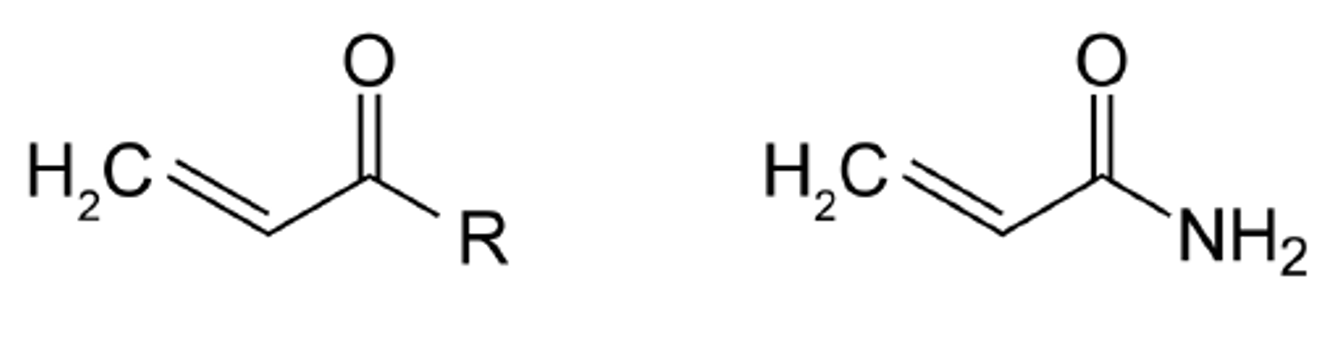
\includegraphics[width=\textwidth]{img/fig/acrylamide.png}
    \caption{Acryloyl group (left) and acrylamide (right)}
    \label{fig:acrylamide} % 2.3
\end{figure}

PAM-solutions undergo hydrolysis, i.e., the reaction of the amide groups of the acrylamide solution with alkaline solutions resulting in carboxylate groups and ammonia. Hydrolysis of acrylamide is shown in Figure \ref{fig:amideHydrol}. The result is a partially hydrolyzed polyacrylamide, HPAM. The degree of hydrolysis, $\tau$ , can be defined as:

\begin{equation}
    \tau = \frac{y}{x+y}
\end{equation}							

where $y$ is the molar concentration of the yielded carboxylate groups and $x$ is the molar concentration amide groups \citep{Al-Muntasheri2012}.

\begin{figure}
    \centering
    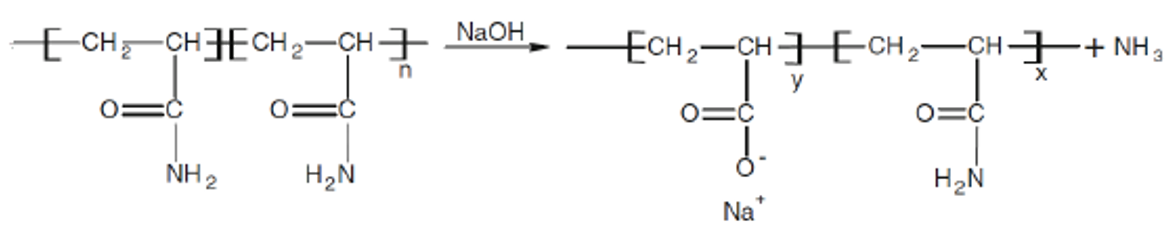
\includegraphics[width=\textwidth]{img/fig/amideHydrol.png}
    \caption{Hydrolysis of amide groups at high pH conditions \citep{Al-muntasheri2008}}
    \label{fig:amideHydrol} % 2.4
\end{figure}

Partially hydrolysation of PAM is important as the negatively charged carboxylate groups are needed to initiate the gelation process in the presence of organic or inorganic cross-linkers. Al-Muntasheri, suggests that there must be at least 1 mol of carboxylate groups before crosslinking can take place. However, there exists an upper limit for hydrolysis that if it is exceeded, the formed gel might either get weaker or precipitate \citep{Al-Muntasheri2007}. When crosslinking is taking place, i.e. the gelation process has been initiated, there exists a threshold value at which the viscoelastic properties dominate the mechanical properties of the polymer solution. At this stage, which is referred to as the sol-gel transition period, the solution is better described as a gel \citep{Albonico1994}.

HPAM requires a cross-linker to undergo gelation. Normally, the gelation time can take several hours, i.e. the time for the gellant (polymer in aqueous state) to become a gel. \cite{Sydansk1993} Sydansk (1993) described a method in the literature to identify the gradual changes observed in the gellant until it becomes a gel, based on its physical behaviour.

These cross-linkers can be either organic or inorganic \citep{Al-Muntasheri2012}. The selection of either type is dependent on the specific type of application and reservoir conditions \citep{Ball1984}. The amount of the added crosslinker to the aqueous solution plays an important role as low amounts of it may result in long term stability issues, and high amounts arise the probability of having syneresis \citep{Sydansk1993, eggert1992}. Syneresis imposes a significant issue as the volume of the formed gel is reduced, secondary channel paths are created, resulting in a failure of the water-diversion application \citep{Al-Muntasheri2007}. However, in general, it has been observed that higher concentrations of cross-linkers result in more viscous gels as shown in Figure \ref{fig:crosslinkerConc}, given that the level of exceeding syneresis threshold is not reached.

\begin{figure}
    \centering
    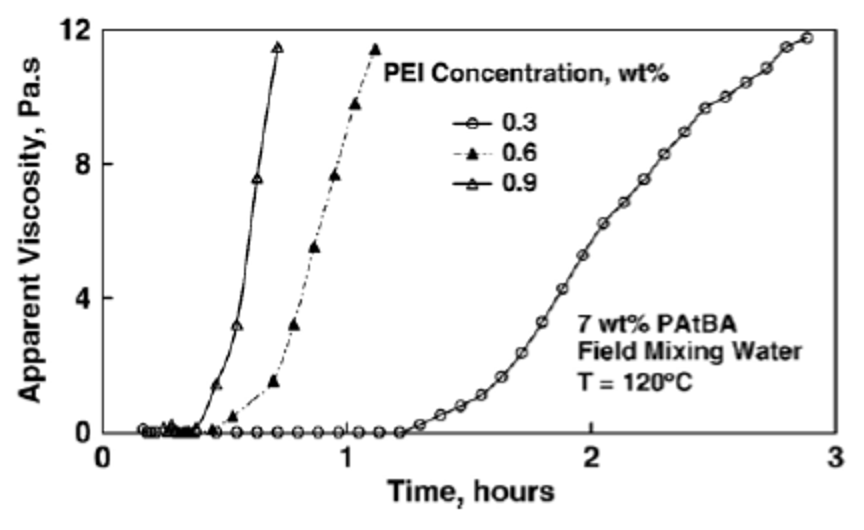
\includegraphics[width=\textwidth]{img/fig/crosslinkerConc.png}
    \caption{Effect of increasing crosslinker (polyetheyleneimine, PEI) concentration on viscosity vs. time \citep{Al-Muntasheri2007}}
    \label{fig:crosslinkerConc} % 2.5
\end{figure}

Inorganic cross-linkers are often referred to as metal crosslinking agents. As the negatively charged (anions) carboxylate groups will chemically bond with the positively charged (cations) cross-linkers, the aforementioned gelation procedure will be initiated. This type of bonding, i.e., ionic bonding, is relatively a weaker type of bonding, as it precipitates at temperatures higher than 75~\celsius, compared with the covalent bond, formed in organic cross-linkers \citep{Al-Muntasheri2005}. Inorganic cross linkers include \ce{Al^3+}, \ce{Zr^4+}, \ce{Cr^3+}, where the latter is the most common cross-linker. Furthermore, \ce{Cr^3+} has the possibility to crosslink biopolymers such as Xanthan which is expensive and difficult to be implemented in large-scale water diversion projects \citep{Al-Muntasheri2012}. However, the application of \ce{Cr^3+} in several countries is limited due to environmental concerns. This will be discussed more in Section \what 2.4.

Organic cross linkers were introduced in the industry in order to overcome the limitation of temperature ranges\citep{Al-Muntasheri2005}. As previously mentioned, covalent bonds are much more stable compared to ionic bonds. Examples of organic cross linkers include aldehydes, phenol-formaldehyde and polyetheyleneimine. The polyacrylamide-phenol/formaldehyde system is a good example on an organically cross-linked gel, and has been reported to withstand the temperature of 121~\celsius~ for about 13 years. However, the use of this gel has been limited due to environmental concerns.

\section{Gel systems behaviour in porous media}

Several gel-systems have different chemical, and physical properties that are needed in the water-diversion applications. Basically, for in-depth water-diversion programs, it is appreciated to use a gel that blocks the high-permeable formation, flows easily through the porous rock before gelation takes place, forms an in-situ highly viscous material that dramatically minimizes the permeability, and shows minimal degradation signs when aged for several years. Retention, deposition, and adsorption are some of the critical parameters that affect the application of a particular gel-system. In this section, the aforementioned properties are discussed.

Particle Transport and Deposition in Porous Media. The behavior of the small-sized particles, e.g., the size of silicate particles to be injected in the reservoir, can be modeled using the classical fine particle transport \citep{Stavland2011}. They discussed several models regarding particle deposition such as Gruesbeck and Collins (1982), Bedrikovetsky et al. (2010), and Guedes et al. (2009). Figure \ref{fig:finesDeposition} shows the deposition of fine particles along the core length (x) using Gruesbeck and Collins simple model. The relative fines concentration, $c/c_0$, can be described as follows:

\begin{equation}
    \frac{c}{c_0} = e^{\frac{-\phi bx}{u}}
\end{equation}

where $\phi$ is the porosity, $b$ is a constant independent of the flowrate, $x$ is the distance, and $u$ is the flowrate. The values used in Figure \ref{fig:finesDeposition} are $\phi = 0.22$ and $b = 1*10^{-5}$ m/s \citep{Stavland2011}. The flowrate is varied as shown in Figure \ref{fig:finesDeposition}, and indicates that at low velocities, higher deposition of particles takes place.

\begin{figure}
    \centering
    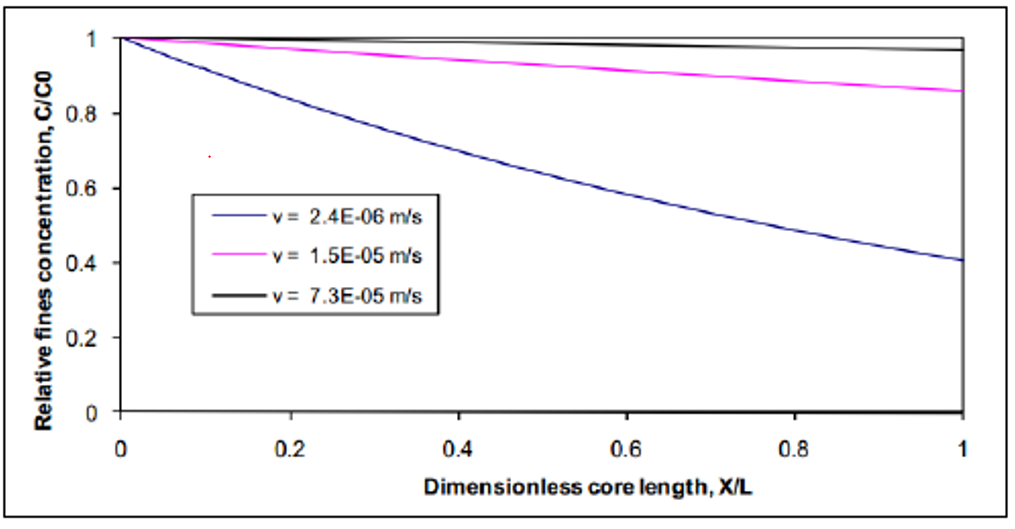
\includegraphics[width=\textwidth]{img/fig/finesDeposition.png}
    \caption{Deposition of fines along the core length \citep{Stavland2011}}
    \label{fig:finesDeposition} % 2.6
\end{figure}

Retention can occur in two different ways, by rock adsorption of the injected polymer solution and possibly also by mechanical entrapment as shown in Figure \ref{fig:retention} \citep{Nabzar1996}. At high velocities, no bridging takes places which is likely due to the high viscous forces \citep{Stavland2011}. As the velocity is decreased, bridging is initiated. Eventually, accumulation takes place, and the pore-throat becomes plugged. In the literature, several authors reported laboratory experiments for gel-system solutions where effect of wettability, mobility reduction, and polymer injection flowrate on retention were examined\citep{Broseta1995, Cohen1986, Idahosa2016}.

\begin{figure}
    \centering
    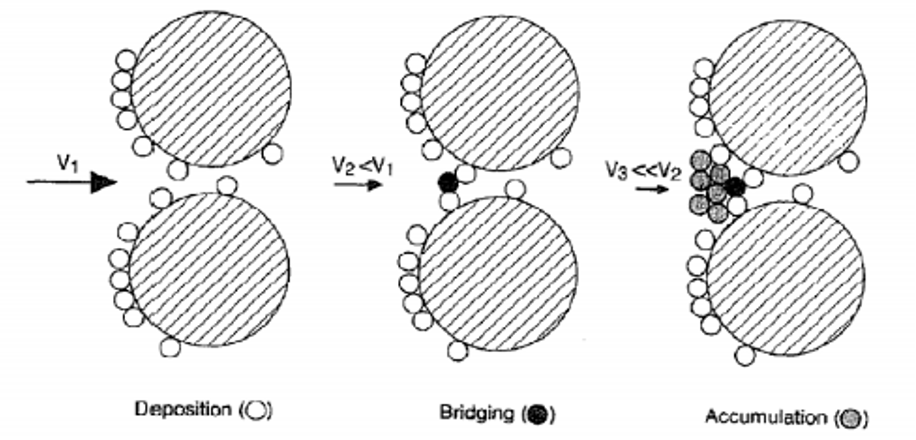
\includegraphics[width=\textwidth]{img/fig/retention.png}
    \caption{Steps of retention at the grain/pore level \citep{Nabzar1996}}
    \label{fig:retention} % 2.7
\end{figure}



\section{Gel systems properties and effects}
There exist several factors that can alter the gelation time, the viscosity as well as the stability of the formed gel-system. These factors include temperature, salinity, pH, and the formation hardness. The main motivation for understanding these effects is to design and select a proper gel-system that is compatible with the reservoir conditions. This section is dedicated solely for polyacrylamide-based polymers properties and effects.

\subsection{Temperature effects}

Reservoir temperature is a major factor that influences the selection criteria of the gel-system to be used in the design of water conformance programs. As discussed earlier, for in-depth water diversion applications, gelation time should be of several weeks, its magnitude depending on characteristics of the reservoir and the nature of the job from an operational standpoint. One of the challenges encountered using Cr3+/HPAM-based polymers is the short gelation times above 60~\celsius~ \citep{Albonico1994}. The use of such gel-systems is possible for near wellbore treatments at low temperature conditions. However, if the temperature is slightly elevated, other considerations should be taken such as the use of un-hydrolyzed PAM and pre-cooling of the near wellbore region \citep{Albonico1994,Al-Muntasheri2012}. Table \ref{tab:gelTimevTemp} shows the gelation times vs temperature for \ce{Cr(acetate)3}/PAM gels.

\begin{table} 
\centering
\caption{Gelation times vs temperature for \ce{Cr(acetate)3}/HPAM gels \citep{Albonico1994}}
\label{tab:gelTimevTemp}
\begin{tabular}{c c } 
\toprule
\textbf{Temperature} & \textbf{Gelation time}\\
~[\celsius] & [hour]\\
\midrule 
60   & 48\\
90   & 2\\ 
120   & $<0.1$\\ 

\bottomrule
\end{tabular}
\end{table}